\newpage
\section{Kiểm thử hệ thống}

\subsection{Kết nối các thiết bị trong cùng VLAN}
Chọn 2 thiết bị trong cùng VLAN:
\begin{figure}[H]
    \centering
    % Điều chỉnh [width=0.9\textwidth] để ảnh chiếm 90% chiều rộng trang giấy
    % Thay "ten_anh_cua_ban.png" bằng tên file ảnh thực tế của bạn
    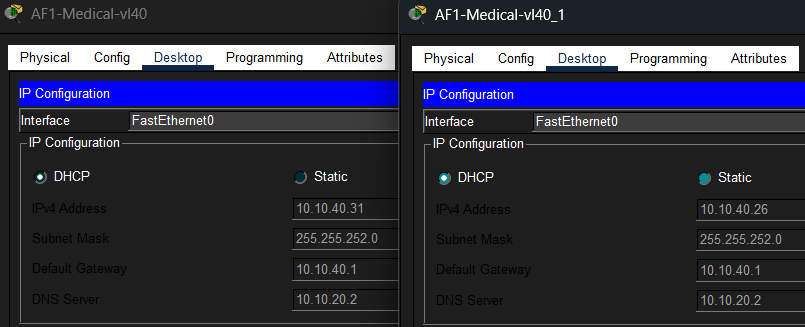
\includegraphics[width=0.8\textwidth]{Pkt_Images/1-2-ip-in-same-LAN.png}
    
    % Tiêu đề của ảnh (giống với caption trong báo cáo mẫu)
    \caption{Địa chỉ IP của 2 thiết bị trong VLAN Medical}
    
    % Nhãn để trích dẫn ảnh trong bài (Ví dụ: "Như được thể hiện trong Hình \ref{fig:three_tier}")
    \label{fig:ip_config_medical}
\end{figure}
\begin{figure}[H]
    \centering
    % Điều chỉnh [width=0.9\textwidth] để ảnh chiếm 90% chiều rộng trang giấy
    % Thay "ten_anh_cua_ban.png" bằng tên file ảnh thực tế của bạn
    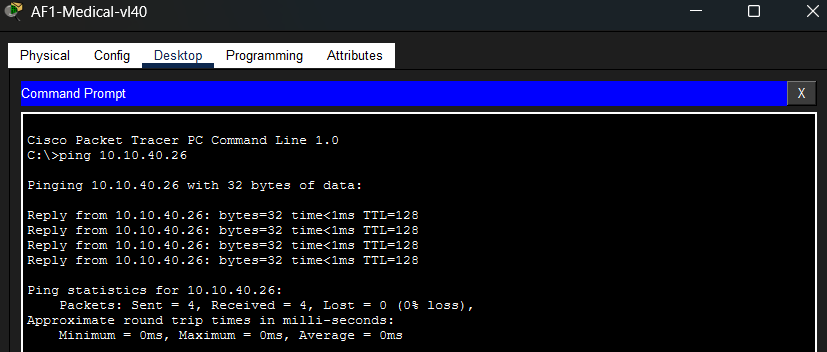
\includegraphics[width=0.8\textwidth]{Pkt_Images/1-ping-success-in-same-VLAN.png}
    
    % Tiêu đề của ảnh (giống với caption trong báo cáo mẫu)
    \caption{Kết quả ping giữa 2 thiết bị trong VLAN Medical}
    
    % Nhãn để trích dẫn ảnh trong bài (Ví dụ: "Như được thể hiện trong Hình \ref{fig:three_tier}")
    \label{fig:medical_to_medical}
\end{figure}

\subsection{Kết nối các thiết bị giữa các VLAN khác nhau}
Chọn 2 thiết bị trong các VLAN khác nhau:
\begin{figure}[H]
    \centering
    % Điều chỉnh [width=0.9\textwidth] để ảnh chiếm 90% chiều rộng trang giấy
    % Thay "ten_anh_cua_ban.png" bằng tên file ảnh thực tế của bạn
    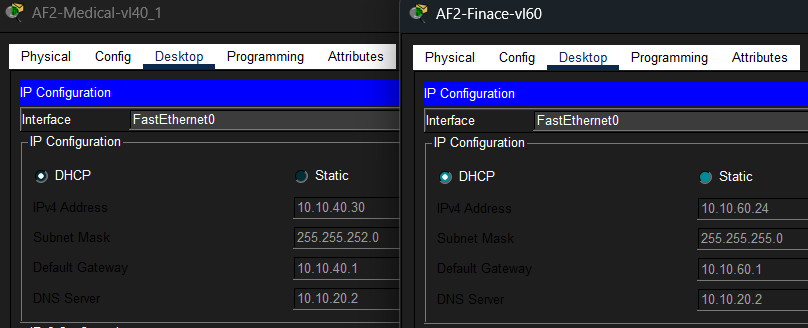
\includegraphics[width=0.8\textwidth]{Pkt_Images/2-2-ip-in-diff-VLAN.png}
    
    % Tiêu đề của ảnh (giống với caption trong báo cáo mẫu)
    \caption{Địa chỉ IP của 2 thiết bị trong VLAN FINANCE và VLAN MEDICAL}
    
    % Nhãn để trích dẫn ảnh trong bài (Ví dụ: "Như được thể hiện trong Hình \ref{fig:three_tier}")
    \label{fig:ip_config_finance}
\end{figure}
\begin{figure}[H]
    \centering
    % Điều chỉnh [width=0.9\textwidth] để ảnh chiếm 90% chiều rộng trang giấy
    % Thay "ten_anh_cua_ban.png" bằng tên file ảnh thực tế của bạn
    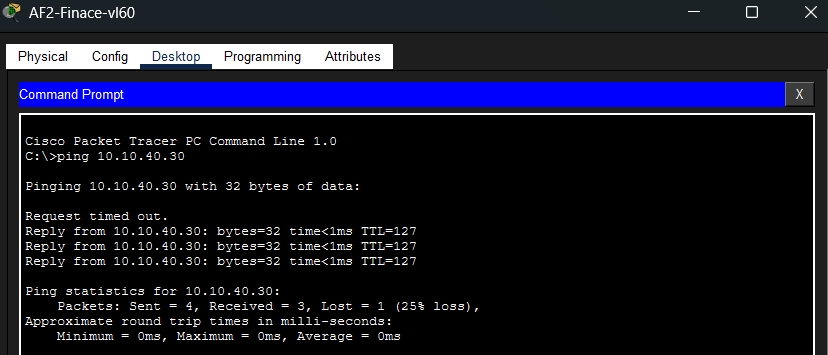
\includegraphics[width=0.8\textwidth]{Pkt_Images/2-ping-success-in-diff-VLAN.png}
    
    % Tiêu đề của ảnh (giống với caption trong báo cáo mẫu)
    \caption{Kết quả ping giữa 2 thiết bị trong VLAN FINANCE và VLAN MEDICAL}
    
    % Nhãn để trích dẫn ảnh trong bài (Ví dụ: "Như được thể hiện trong Hình \ref{fig:three_tier}")
    \label{fig:hr_to_finance}
\end{figure}
\subsection{Kết nối các thiết bị giữa trụ sở chính và hai trụ sở phụ}
\begin{figure}[H]
    \centering
    % Điều chỉnh [width=0.9\textwidth] để ảnh chiếm 90% chiều rộng trang giấy
    % Thay "ten_anh_cua_ban.png" bằng tên file ảnh thực tế của bạn
    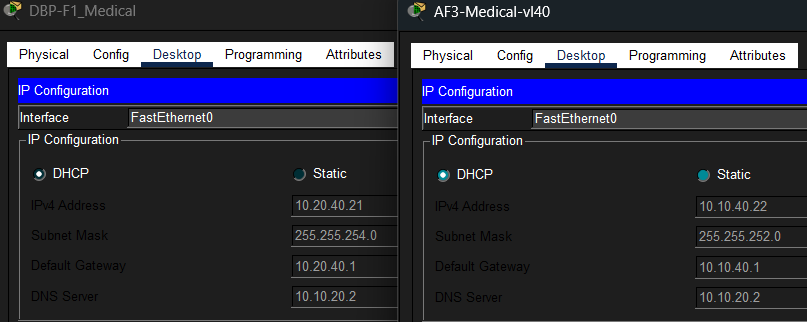
\includegraphics[width=0.8\textwidth]{Pkt_Images/3-2-ip-diff-site.png}
    
    % Tiêu đề của ảnh (giống với caption trong báo cáo mẫu)
    \caption{Địa chỉ IP của thiết bị tại trụ sở chính và thiết bị tại trụ sở DBP}
    
    % Nhãn để trích dẫn ảnh trong bài (Ví dụ: "Như được thể hiện trong Hình \ref{fig:three_tier}")
    \label{fig:ip_config_dbp_main}
\end{figure}
\begin{figure}[H]
    \centering
    % Điều chỉnh [width=0.9\textwidth] để ảnh chiếm 90% chiều rộng trang giấy
    % Thay "ten_anh_cua_ban.png" bằng tên file ảnh thực tế của bạn
    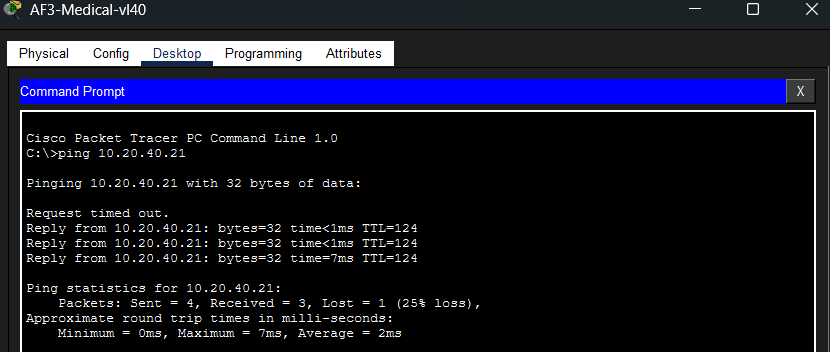
\includegraphics[width=0.8\textwidth]{Pkt_Images/3-ping-success.png}
    
    % Tiêu đề của ảnh (giống với caption trong báo cáo mẫu)
    \caption{Kết quả ping giữa thiết bị tại trụ sở chính và thiết bị tại trụ sở DBP}
    
    % Nhãn để trích dẫn ảnh trong bài (Ví dụ: "Như được thể hiện trong Hình \ref{fig:three_tier}")
    \label{fig:main_to_dbp}
\end{figure}
\subsection{Kết nối đến server DMZ}
\begin{figure}[H]
    \centering
    % Điều chỉnh [width=0.9\textwidth] để ảnh chiếm 90% chiều rộng trang giấy
    % Thay "ten_anh_cua_ban.png" bằng tên file ảnh thực tế của bạn
    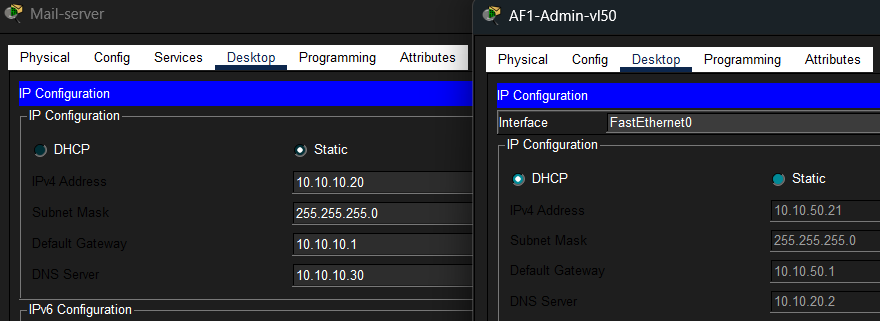
\includegraphics[width=0.8\textwidth]{Pkt_Images/4-2-ip.png}
    
    % Tiêu đề của ảnh (giống với caption trong báo cáo mẫu)
    \caption{Địa chỉ IP của Mail Server trong DMZ và đia chỉ IP của thiết bị trong VLAN ADMIN}
    
    % Nhãn để trích dẫn ảnh trong bài (Ví dụ: "Như được thể hiện trong Hình \ref{fig:three_tier}")
    \label{fig:ip_config_mailserver}
\end{figure}
\begin{figure}[H]
    \centering
    % Điều chỉnh [width=0.9\textwidth] để ảnh chiếm 90% chiều rộng trang giấy
    % Thay "ten_anh_cua_ban.png" bằng tên file ảnh thực tế của bạn
    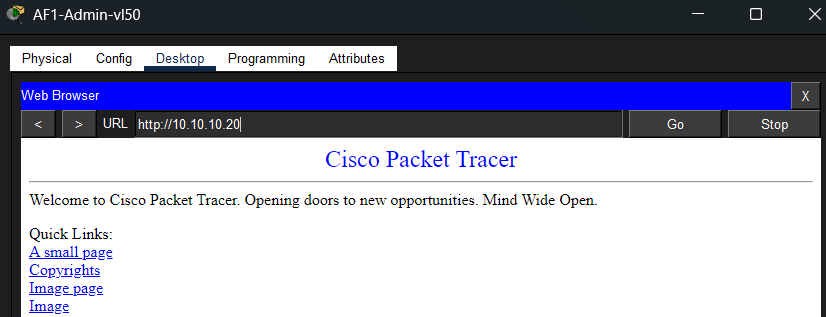
\includegraphics[width=0.8\textwidth]{Pkt_Images/4-mail-server.png}
    
    % Tiêu đề của ảnh (giống với caption trong báo cáo mẫu)
    \caption{Truy cập Mail server từ trình duyệt của thiết bị (Web Server) trong VLAN ADMIN}
    
    % Nhãn để trích dẫn ảnh trong bài (Ví dụ: "Như được thể hiện trong Hình \ref{fig:three_tier}")
    \label{fig:admin_to_mailserver}
\end{figure}
\begin{figure}[H]
    \centering
    % Điều chỉnh [width=0.9\textwidth] để ảnh chiếm 90% chiều rộng trang giấy
    % Thay "ten_anh_cua_ban.png" bằng tên file ảnh thực tế của bạn
    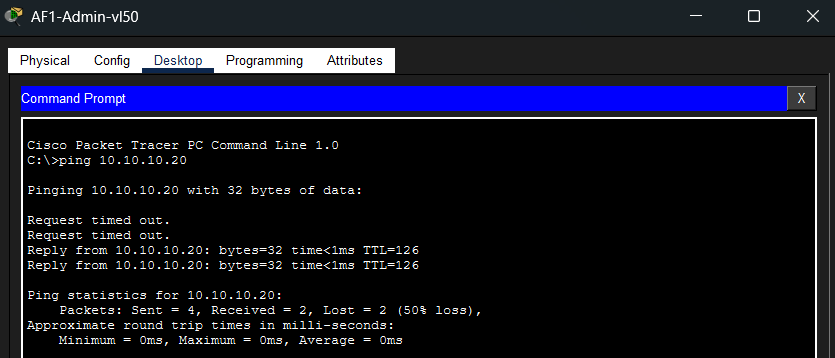
\includegraphics[width=0.8\textwidth]{Pkt_Images/4-ping-success.png}
    
    % Tiêu đề của ảnh (giống với caption trong báo cáo mẫu)
    \caption{Kết quả ping từ thiết bị trong VLAN ADMIN đến Mail Server trong DMZ}
    
    % Nhãn để trích dẫn ảnh trong bài (Ví dụ: "Như được thể hiện trong Hình \ref{fig:three_tier}")
    \label{fig:admin_to_mailserver}
\end{figure}

\subsection{Chặn truy cập từ GUEST đến các VLAN nội bộ}
\begin{figure}[H]
    \centering
    % Điều chỉnh [width=0.9\textwidth] để ảnh chiếm 90% chiều rộng trang giấy
    % Thay "ten_anh_cua_ban.png" bằng tên file ảnh thực tế của bạn
    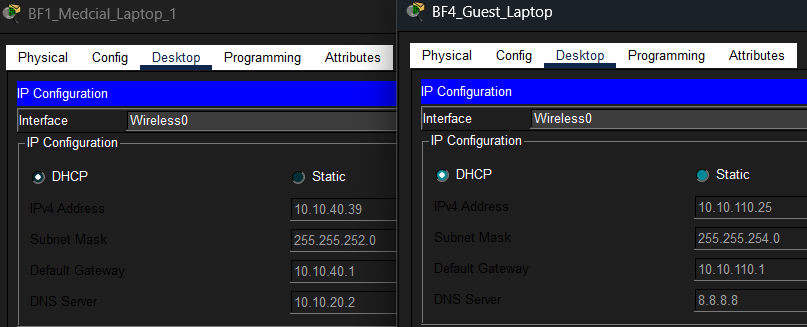
\includegraphics[width=0.8\textwidth]{Pkt_Images/5-2-ip.png}
    
    % Tiêu đề của ảnh (giống với caption trong báo cáo mẫu)
    \caption{Địa chỉ IP của thiết bị trong VLAN GUEST và thiết bị trong VLAN MEDICAL(tại trụ sở chính)}
    
    % Nhãn để trích dẫn ảnh trong bài (Ví dụ: "Như được thể hiện trong Hình \ref{fig:three_tier}")
    \label{fig:ip_config_medical_2}
\end{figure}
\begin{figure}[H]
    \centering
    % Điều chỉnh [width=0.9\textwidth] để ảnh chiếm 90% chiều rộng trang giấy
    % Thay "ten_anh_cua_ban.png" bằng tên file ảnh thực tế của bạn
    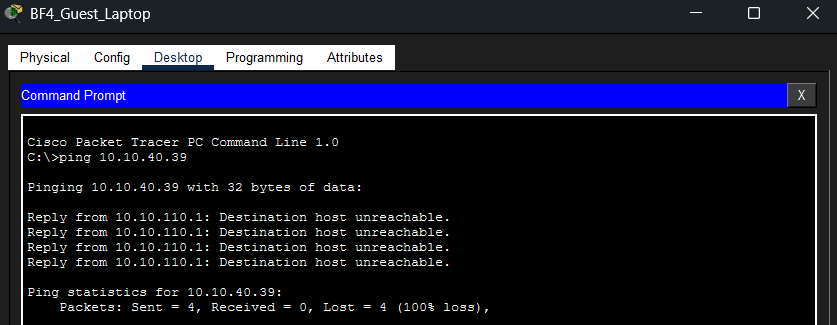
\includegraphics[width=0.8\textwidth]{Pkt_Images/5-ping-fail.png}
    
    % Tiêu đề của ảnh (giống với caption trong báo cáo mẫu)
    \caption{Kết quả ping từ thiết bị trong VLAN GUEST đến thiết bị trong VLAN MEDICAL tại trụ sở chính}
    
    % Nhãn để trích dẫn ảnh trong bài (Ví dụ: "Như được thể hiện trong Hình \ref{fig:three_tier}")
    \label{fig:guest_to_medical}
\end{figure}
\begin{figure}[H]
    \centering
    % Điều chỉnh [width=0.9\textwidth] để ảnh chiếm 90% chiều rộng trang giấy
    % Thay "ten_anh_cua_ban.png" bằng tên file ảnh thực tế của bạn
    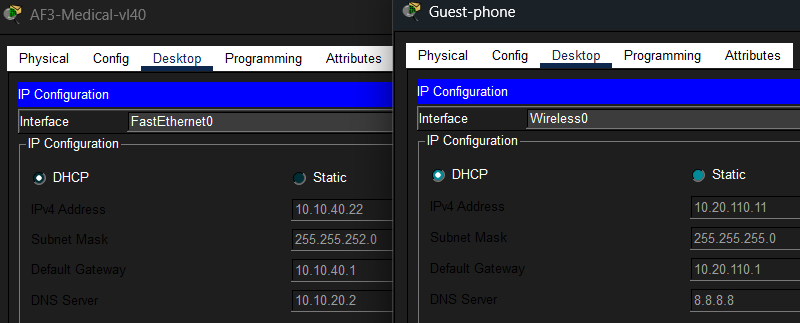
\includegraphics[width=0.8\textwidth]{Pkt_Images/5-ip-MAIN-DBP-site.png}
    
    % Tiêu đề của ảnh (giống với caption trong báo cáo mẫu)
    \caption{Địa chỉ IP của thiết bị trong VLAN GUEST(tại trụ sở DBP) và thiết bị trong VLAN MEDICAL(tại trụ sở chính)}
    
    % Nhãn để trích dẫn ảnh trong bài (Ví dụ: "Như được thể hiện trong Hình \ref{fig:three_tier}")
    \label{fig:ip_config_medical_3}
\end{figure}
\begin{figure}[H]
    \centering
    % Điều chỉnh [width=0.9\textwidth] để ảnh chiếm 90% chiều rộng trang giấy
    % Thay "ten_anh_cua_ban.png" bằng tên file ảnh thực tế của bạn
    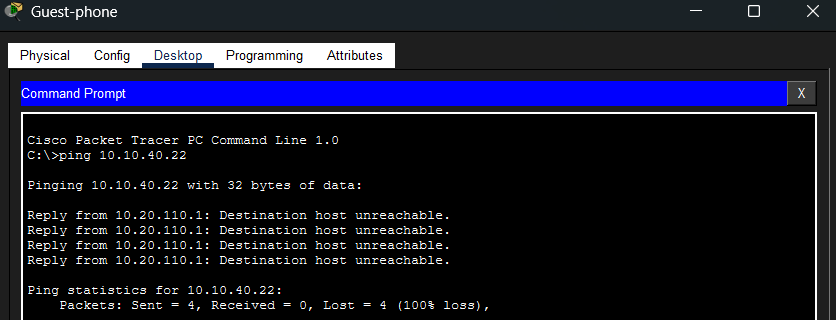
\includegraphics[width=0.8\textwidth]{Pkt_Images/5-ping-fail-DBP-site.png}
    
    % Tiêu đề của ảnh (giống với caption trong báo cáo mẫu)
    \caption{Kết quả ping từ thiết bị trong VLAN GUEST(tại trụ sở DBP) đến thiết bị trong VLAN MEDICAL (tại trụ sở chính)}
    
    % Nhãn để trích dẫn ảnh trong bài (Ví dụ: "Như được thể hiện trong Hình \ref{fig:three_tier}")
    \label{fig:guest_to_medical_1}
\end{figure}
\subsection{Kết nối Internet đến Webserver}
\textbf{Tại trụ sở chính:}
\begin{figure}[H]
    \centering
    % Điều chỉnh [width=0.9\textwidth] để ảnh chiếm 90% chiều rộng trang giấy
    % Thay "ten_anh_cua_ban.png" bằng tên file ảnh thực tế của bạn
    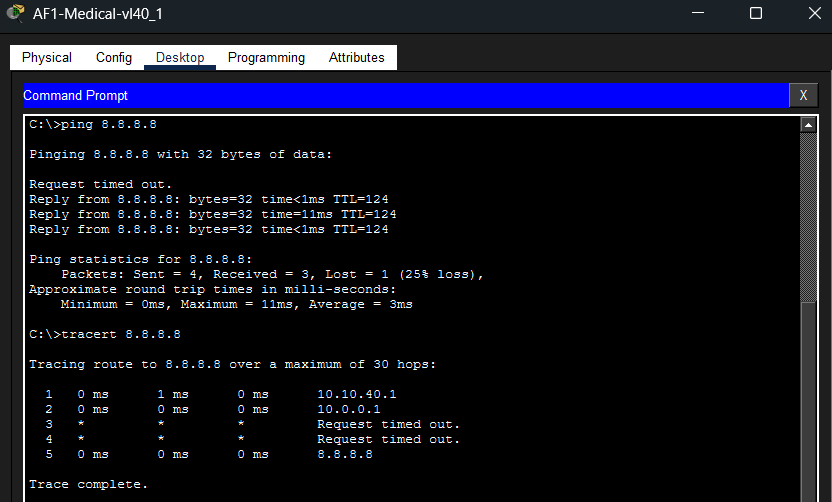
\includegraphics[width=0.8\textwidth]{Pkt_Images/6-Main-to-Internet.png}
    
    % Tiêu đề của ảnh (giống với caption trong báo cáo mẫu)
    \caption{Kết quả ping từ thiết bị trong VLAN MEDICAL (tại cơ sở chính) đến địa chỉ IP public của Internet}
    % Nhãn để trích dẫn ảnh trong bài (Ví dụ: "Như được thể hiện trong Hình \ref{fig:three_tier}")
    \label{fig:ip_main_to_internet}
\end{figure}
\begin{figure}[H]
    \centering
    % Điều chỉnh [width=0.9\textwidth] để ảnh chiếm 90% chiều rộng trang giấy
    % Thay "ten_anh_cua_ban.png" bằng tên file ảnh thực tế của bạn
    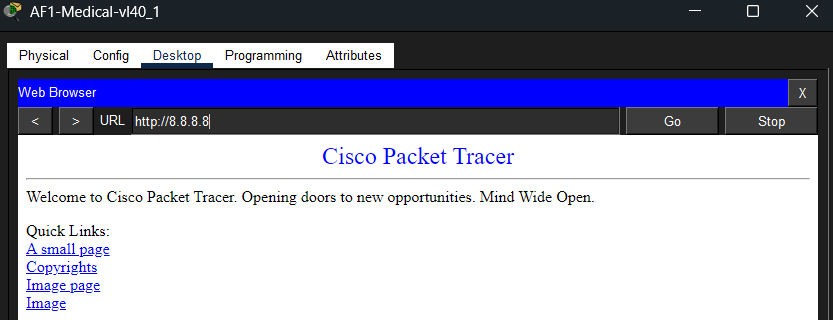
\includegraphics[width=0.8\textwidth]{Pkt_Images/6-Main-webserver.png}
    
    % Tiêu đề của ảnh (giống với caption trong báo cáo mẫu)
    \caption{Truy cập Webserver từ thiết bị trong VLAN MEDICAL qua Internet}
    
    % Nhãn để trích dẫn ảnh trong bài (Ví dụ: "Như được thể hiện trong Hình \ref{fig:three_tier}")
    \label{fig:main_to_internet_1}
\end{figure}
\textbf{Tại trụ sở BHTQ:}
\begin{figure}[H]
    \centering
    % Điều chỉnh [width=0.9\textwidth] để ảnh chiếm 90% chiều rộng trang giấy
    % Thay "ten_anh_cua_ban.png" bằng tên file ảnh thực tế của bạn
    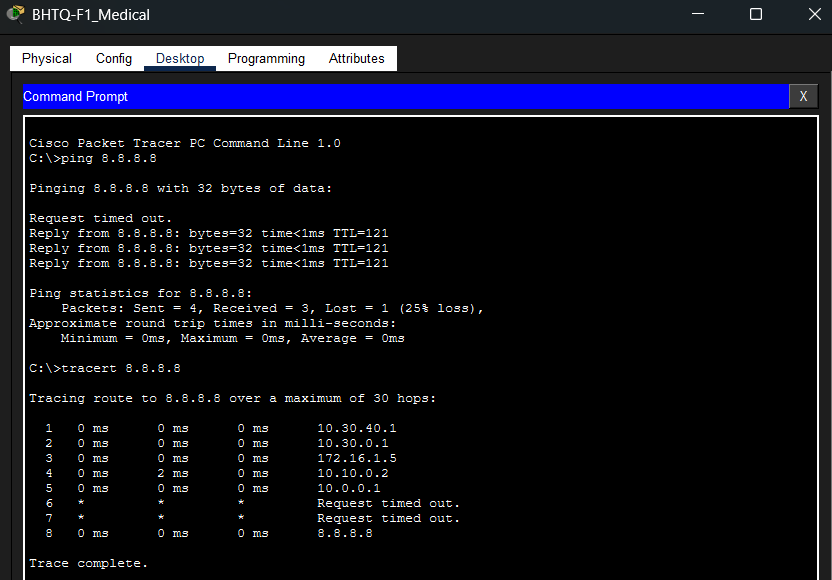
\includegraphics[width=0.8\textwidth]{Pkt_Images/6-BHTQ-to-Internet.png}
    
    % Tiêu đề của ảnh (giống với caption trong báo cáo mẫu)
    \caption{Kết quả ping từ thiết bị trong VLAN MEDICAL (tại cơ sở BHTQ) đến địa chỉ IP public của Internet}
    % Nhãn để trích dẫn ảnh trong bài (Ví dụ: "Như được thể hiện trong Hình \ref{fig:three_tier}")
    \label{fig:ip_bhtq_to_internet}
\end{figure}
\begin{figure}[H]
    \centering
    % Điều chỉnh [width=0.9\textwidth] để ảnh chiếm 90% chiều rộng trang giấy
    % Thay "ten_anh_cua_ban.png" bằng tên file ảnh thực tế của bạn
    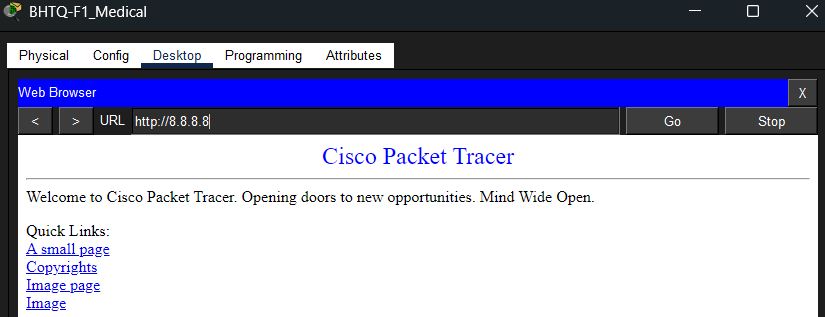
\includegraphics[width=0.8\textwidth]{Pkt_Images/6-BHTQ-webserver.png}
    
    % Tiêu đề của ảnh (giống với caption trong báo cáo mẫu)
    \caption{Truy cập Webserver từ thiết bị trong VLAN MEDICAL qua Internet}
    
    % Nhãn để trích dẫn ảnh trong bài (Ví dụ: "Như được thể hiện trong Hình \ref{fig:three_tier}")
    \label{fig:bhtq_to_internet_1}
\end{figure}

\subsection{Quản lý Camera}
\begin{figure}[H]
    \centering
    % Điều chỉnh [width=0.9\textwidth] để ảnh chiếm 90% chiều rộng trang giấy
    % Thay "ten_anh_cua_ban.png" bằng tên file ảnh thực tế của bạn
    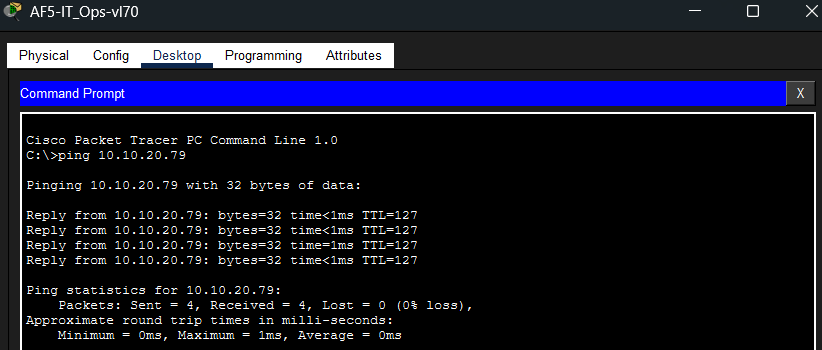
\includegraphics[width=0.8\textwidth]{Pkt_Images/7-ping-server-IoT.png}
    
    % Tiêu đề của ảnh (giống với caption trong báo cáo mẫu)
    \caption{Kết quả ping từ thiết bị trong VLAN IT-OPS đến Server IoT camera trong VLAN SERVER-FARM}
    
    % Nhãn để trích dẫn ảnh trong bài (Ví dụ: "Như được thể hiện trong Hình \ref{fig:three_tier}")
    \label{fig:ping_it_ops_to_iot}
\end{figure}
\begin{figure}[H]
    \centering
    % Điều chỉnh [width=0.9\textwidth] để ảnh chiếm 90% chiều rộng trang giấy
    % Thay "ten_anh_cua_ban.png" bằng tên file ảnh thực tế của bạn
    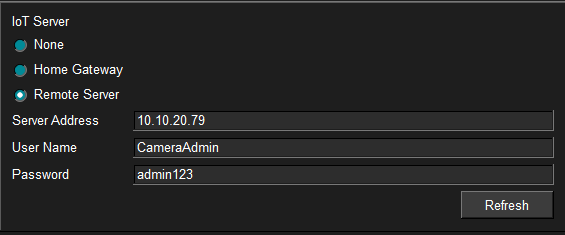
\includegraphics[width=1\textwidth]{Pkt_Images/7-username-pw.png}
    
    % Tiêu đề của ảnh (giống với caption trong báo cáo mẫu)
    \caption{Thông tin đăng nhập vào Server IoT camera}
    
    % Nhãn để trích dẫn ảnh trong bài (Ví dụ: "Như được thể hiện trong Hình \ref{fig:three_tier}")
    \label{fig:iot_username_password}
\end{figure}
\begin{figure}[H]
    \centering
    % Điều chỉnh [width=0.9\textwidth] để ảnh chiếm 90% chiều rộng trang giấy
    % Thay "ten_anh_cua_ban.png" bằng tên file ảnh thực tế của bạn
    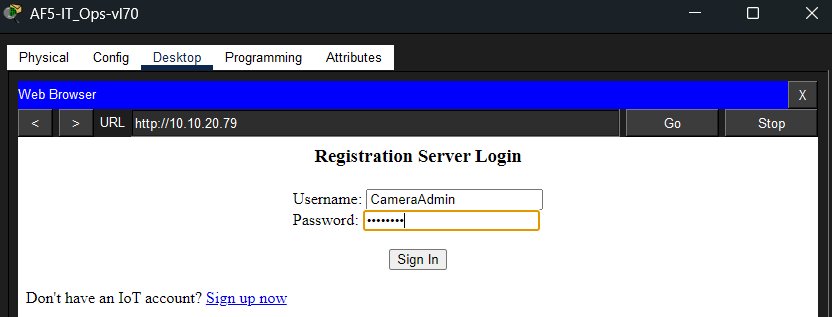
\includegraphics[width=0.8\textwidth]{Pkt_Images/7-sign-in.png}
    
    % Tiêu đề của ảnh (giống với caption trong báo cáo mẫu)
    \caption{Đăng nhập vào Server IoT camera từ thiết bị trong VLAN IT-OPS}
    
    % Nhãn để trích dẫn ảnh trong bài (Ví dụ: "Như được thể hiện trong Hình \ref{fig:three_tier}")
    \label{fig:it_ops_to_iot_1}
\end{figure}
\begin{figure}[H]
    \centering
    % Điều chỉnh [width=0.9\textwidth] để ảnh chiếm 90% chiều rộng trang giấy
    % Thay "ten_anh_cua_ban.png" bằng tên file ảnh thực tế của bạn
    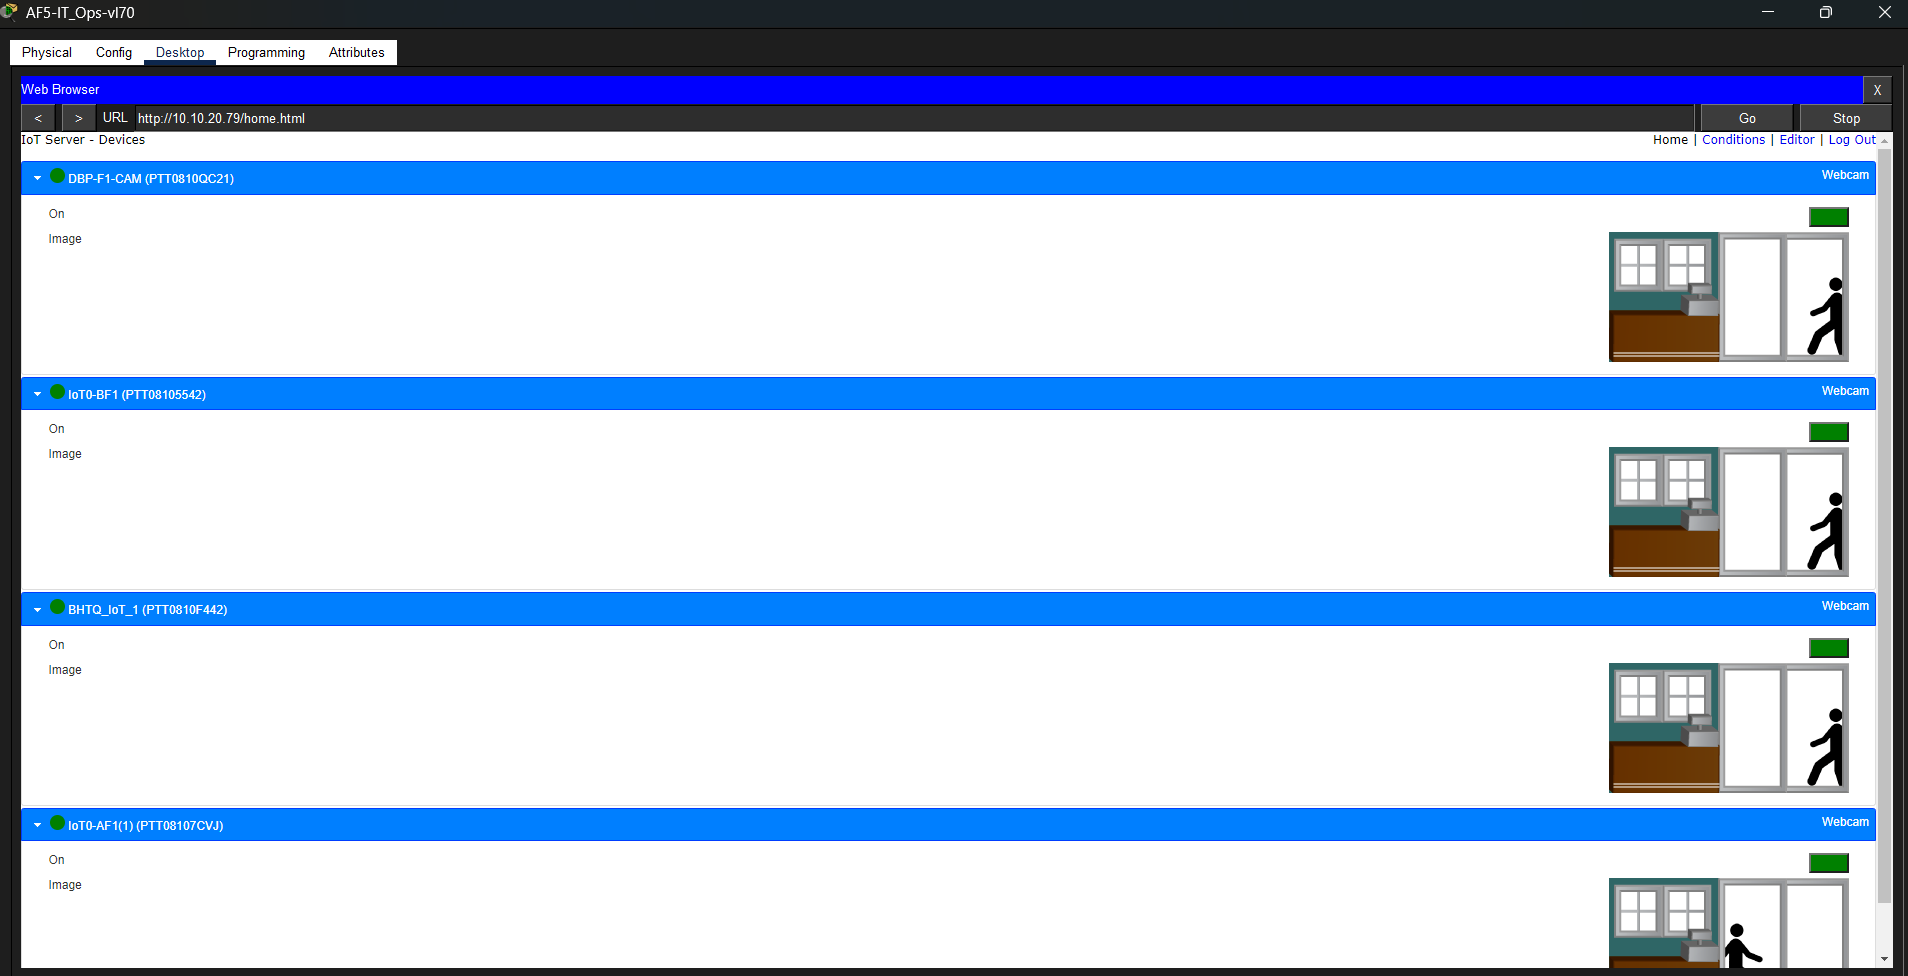
\includegraphics[width=0.8\textwidth]{Pkt_Images/7-web-server.png}
    
    % Tiêu đề của ảnh (giống với caption trong báo cáo mẫu)
    \caption{Theo dõi camera từ thiết bị trong VLAN IT-OPS}
    
    % Nhãn để trích dẫn ảnh trong bài (Ví dụ: "Như được thể hiện trong Hình \ref{fig:three_tier}")
    \label{fig:it_ops_to_iot_2}
\end{figure}
\subsection{Kết nối từ Teleworker đến các VLAN nội bộ}  
\begin{figure}[H]
    \centering
    % Điều chỉnh [width=0.9\textwidth] để ảnh chiếm 90% chiều rộng trang giấy
    % Thay "ten_anh_cua_ban.png" bằng tên file ảnh thực tế của bạn
    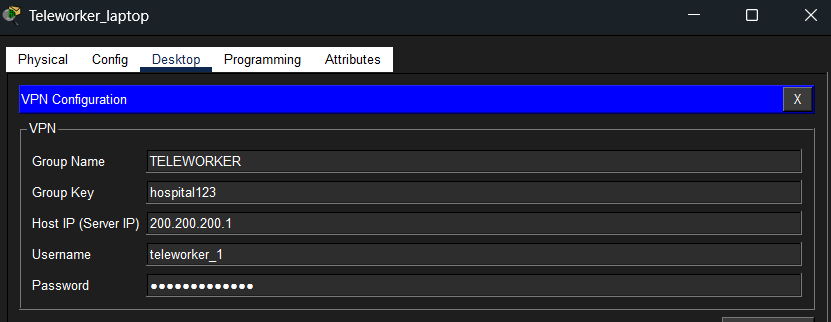
\includegraphics[width=0.8\textwidth]{Pkt_Images/8-access-VPN.png}
    
    % Tiêu đề của ảnh (giống với caption trong báo cáo mẫu)
    \caption{Thiết lập kết nối VPN từ thiết bị của Teleworker đến Firewall tại trụ sở chính}
    
    % Nhãn để trích dẫn ảnh trong bài (Ví dụ: "Như được thể hiện trong Hình \ref{fig:three_tier}")
    \label{fig:teleworker_vpn}
\end{figure}
\begin{figure}[H]
    \centering
    % Điều chỉnh [width=0.9\textwidth] để ảnh chiếm 90% chiều rộng trang giấy
    % Thay "ten_anh_cua_ban.png" bằng tên file ảnh thực tế của bạn
    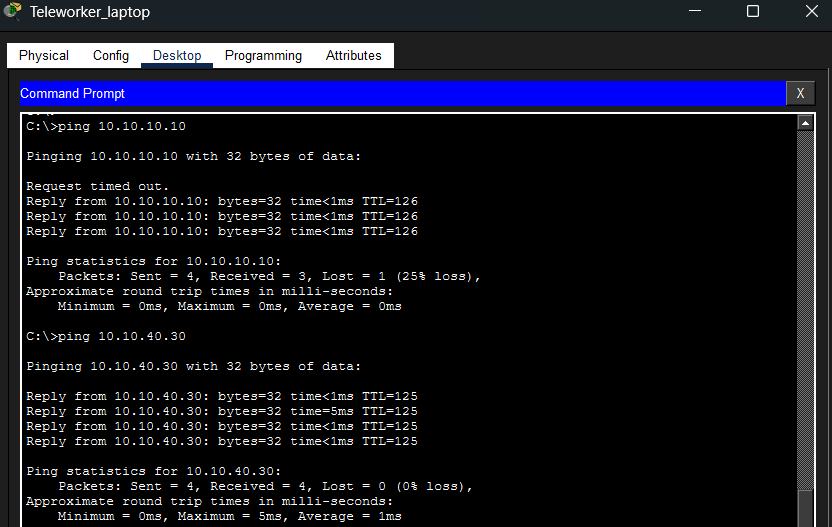
\includegraphics[width=0.8\textwidth]{Pkt_Images/8-ping-success.png}
    
    % Tiêu đề của ảnh (giống với caption trong báo cáo mẫu)
    \caption{Kết quả ping từ thiết bị của Teleworker đến thiết bị trong VLAN MEDICAL tại trụ sở chính và Webserver trong DMZ}
    
    % Nhãn để trích dẫn ảnh trong bài (Ví dụ: "Như được thể hiện trong Hình \ref{fig:three_tier}")
    \label{fig:tele_to_inter_vlan}
\end{figure}